\documentclass[informe.tex]{subfiles}
\begin{document}

\textbf{Implentación realizada utilizando Microcontrolador}\newline

El montaje completo consiste de una placa embebida de bajo costo, una interfaz para la grabación y depuración del código en el microcontrolador, un circuito para proteger las entrada analógica, y un circuito de salida que actúa como carga, Fig.  \ref{fig:disenio_y_construccion:stm32:board}.

\begin{figure}[h!]
	\centering
	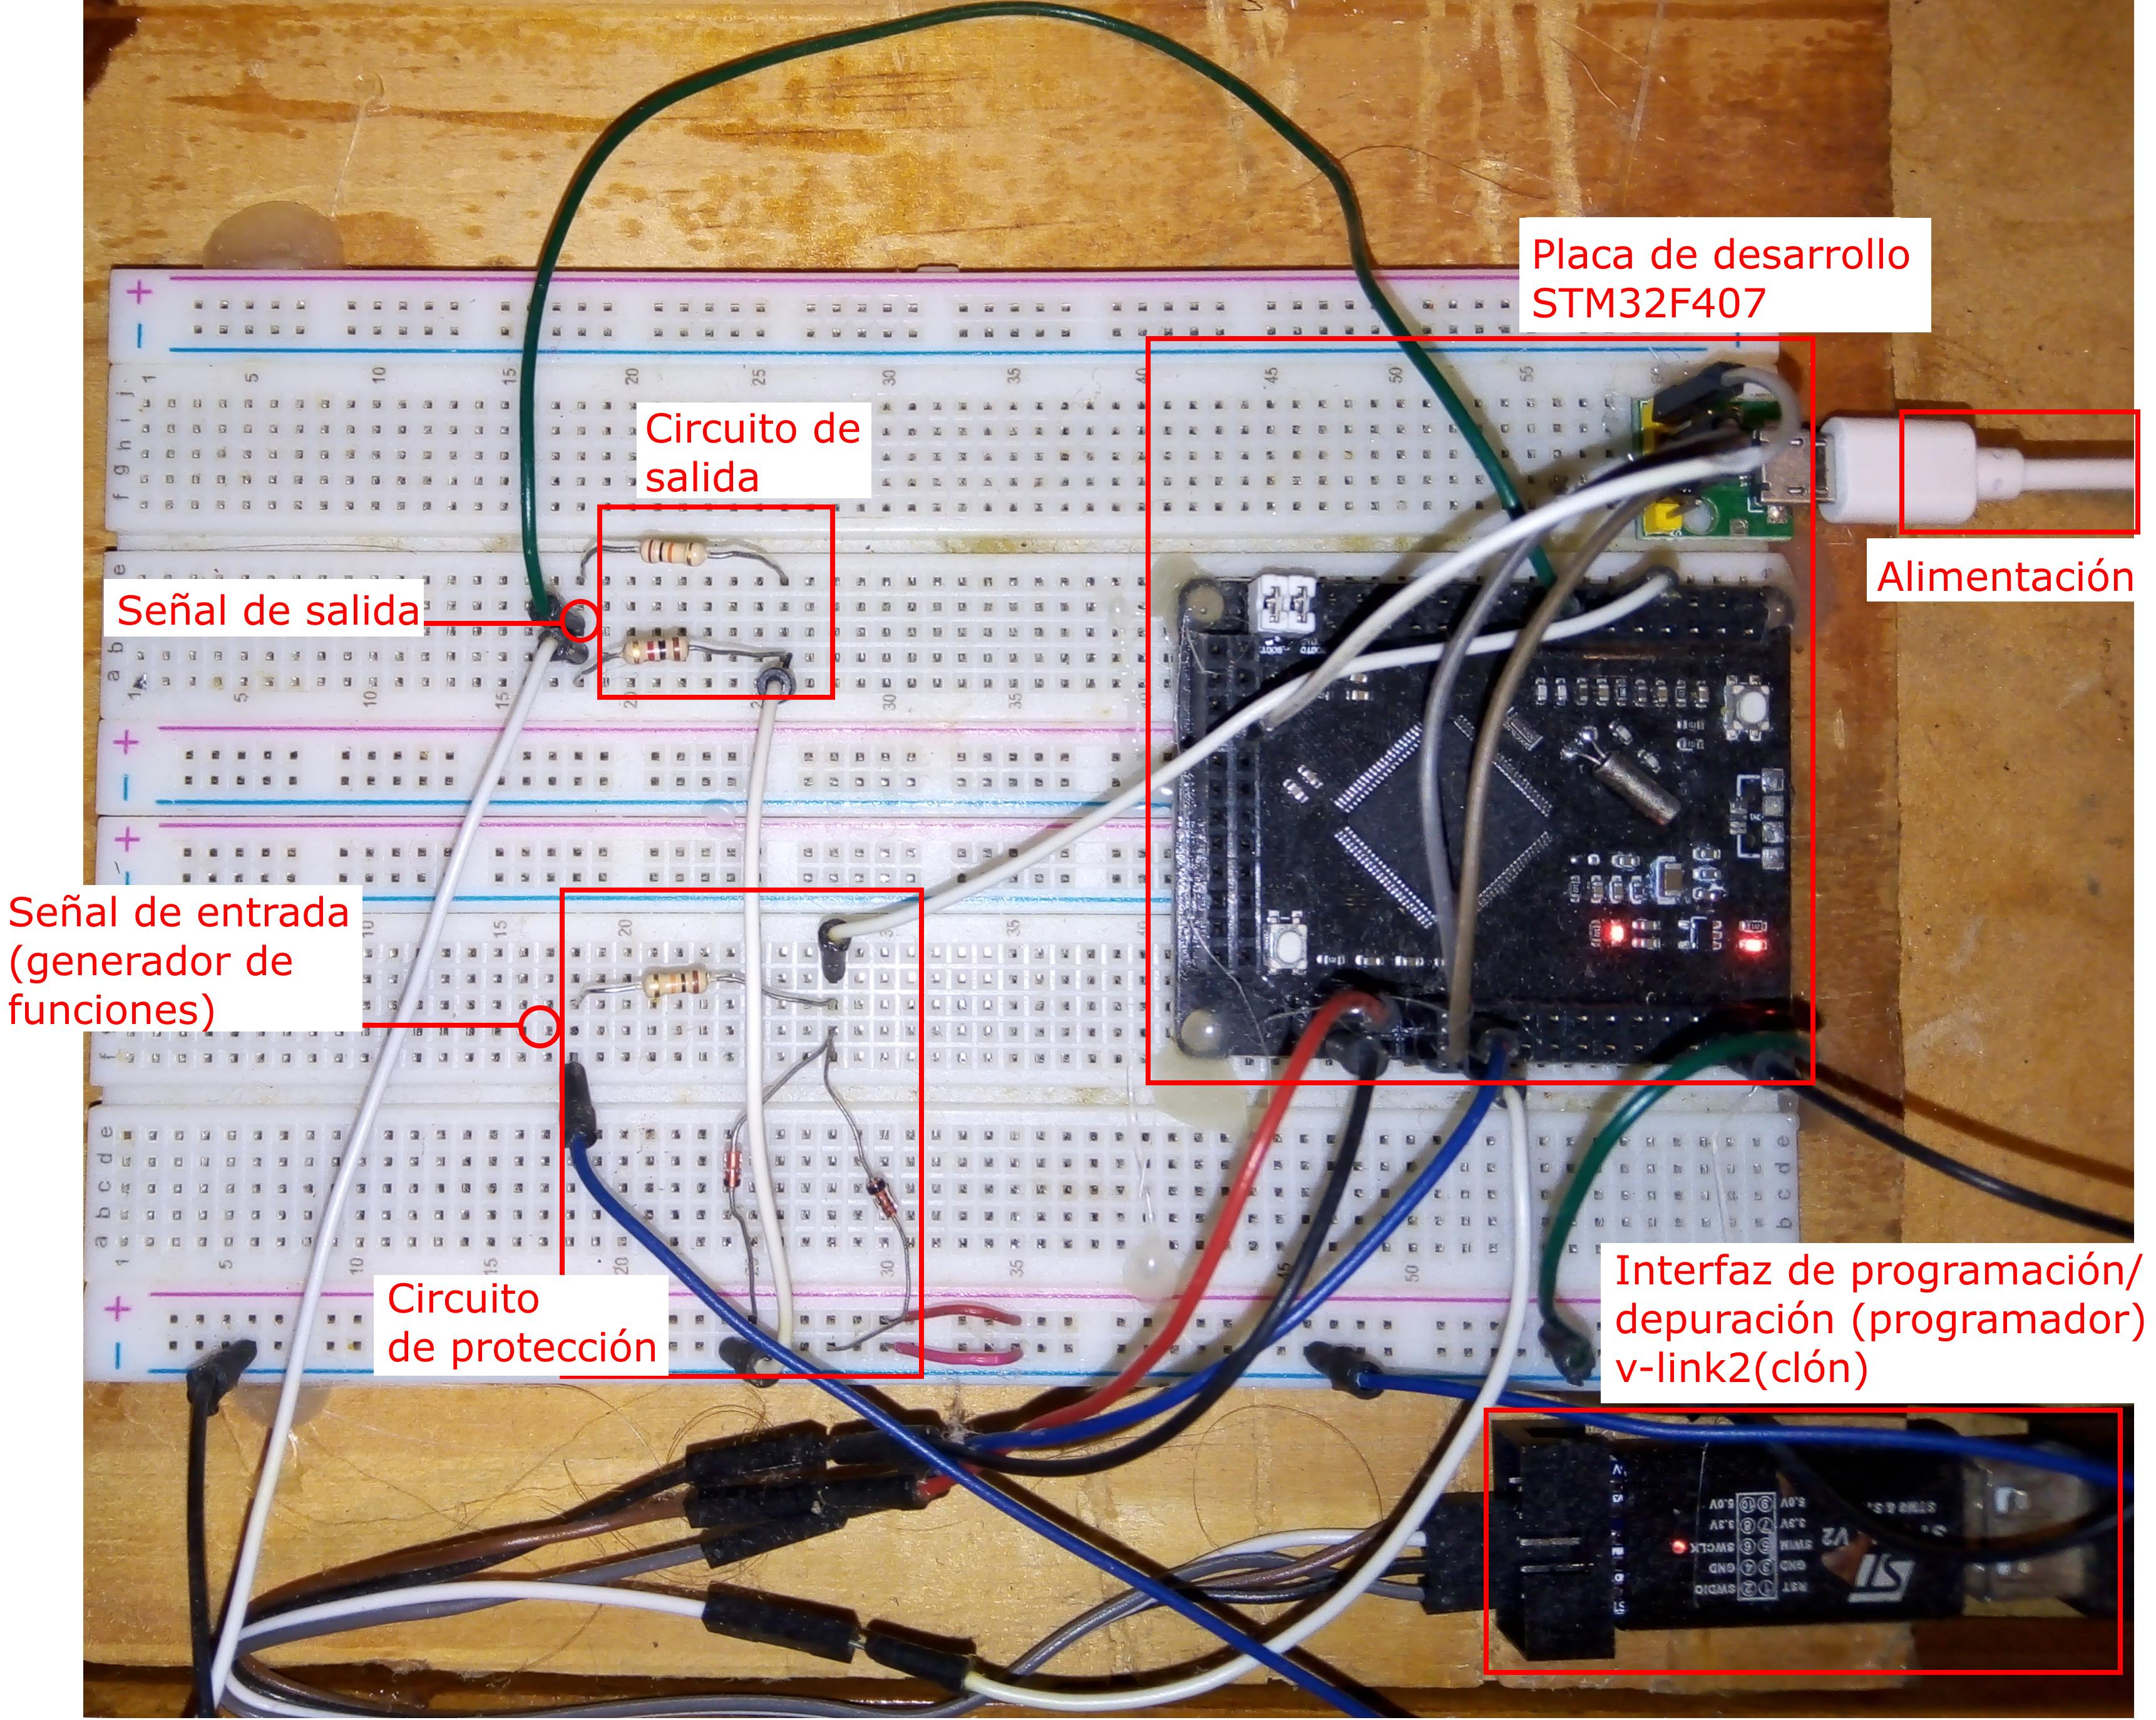
\includegraphics[scale=0.13]{foto_stm32f407_board.jpg}	
	\caption{Montaje del sistema embebido con microcontrolador}
	\label{fig:disenio_y_construccion:stm32:board}
	\end{figure}

Las características generales del microcontrolador de interés que posee la placa embebida para esta aplicación son:\\
- La denominación comercial del microcontrolador es STM32F407VGT.\\ 
- La CPU es de arquitectura ARM, Corte-M4-32 bits, con una señal de reloj de sistema máxima de 168 MHz.\\
- El rango de voltaje de alimentación es de 1.8 de 3.3V (valor típico).\\
- El módulo de conversión analógica-digital, ADC, incluido: tiene 3 unidades de 12-bit, con un voltaje máximo de entrada menor o igual al voltaje de alimentación, y la tasa de muestreo ronda entre 2 a 6 MSPS, este valor de operación es dependiente de la alimentación y de su configuración; la impedancia de entrada es de 50 k$\Omega$, el valor de resistencia de muestreo es de 6 k$\Omega$ y el capacitor de muestreo es  aproximadamente de 4 $pF$.\\
- El módulo de conversión digital-analógica, DAC, incluido: tiene dos unidades. Cada uno tiene una resistencia de carga de 5K$\Omega$, eso es si tiene el buffer de salida activado, una impedancia de salida de 15 k$\Omega$ y una capacitancia parásita de 50 $pF$.\\
- El módulo de temporización incluido, Timer: tiene 17 unidades, hay de 16 bits y de 32 bits, con frecuencia de operación máxima de 168 MHz.\\

La arquitectura de la implementación del sistema embebido para el desarrollo de los filtros digitales se puede resumir en la Fig. \ref{fig:disenio_y_construccion:stm32:arq}.\\
\begin{figure}[h]
	\centering
	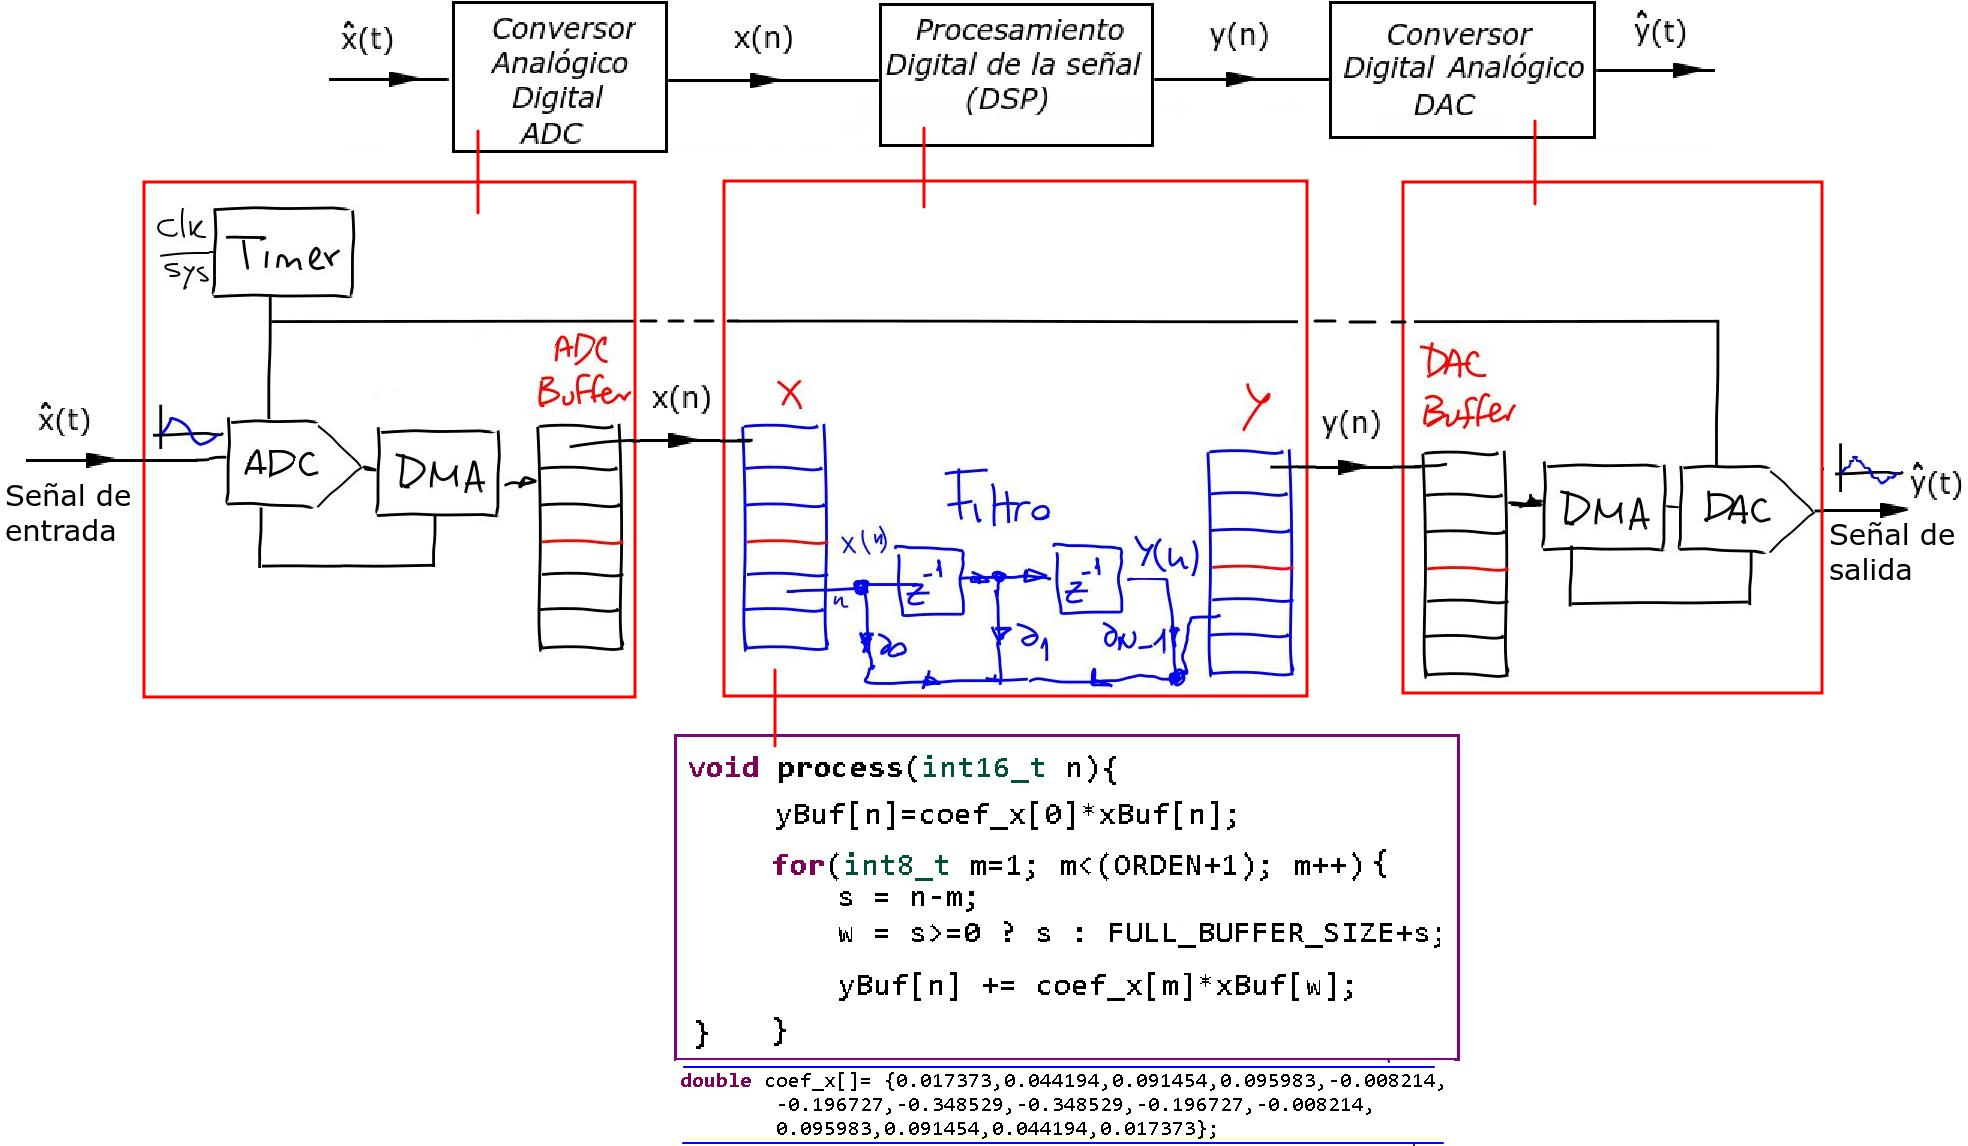
\includegraphics[scale=0.33]{construccion_bloques_micro.jpg}	
	\caption{Representación en bloques de la arquitectura desarrollada para los filtros digitales por medio de microcontrolador}
	\label{fig:disenio_y_construccion:stm32:arq}
	\end{figure}
El Timer es simplemente un contador que toma la señal de reloj del bus interno del microcontrolador al que está conectado, y a partir del valor de la cuenta cargado en el registro de comparación genera señales de menor frecuencia. El principio de funcionamiento consiste en iniciar un registro de comparación y cuando el contador desborda o llega al valor de comparación precargado genera una señal de activación y luego se reinicia para generar otro ciclo de cuenta. En este caso, se genera una señal para disparar el inicio de conversión del módulo ADC y del módulo DAC. La frecuencia de esta señal de control se considera la frecuencia de muestreo.\newline

El cálculo del valor que configurará en el registro de comparación del Timer va a determinar la frecuencia de muestreo utilizada. Éste valor de registro va a depender de la frecuencia de la señal de reloj del bus que alimenta al Timer en cuestión (en este caso $freq_{bus}=84 MHz$), a esta frecuencia se la divide por la cantidad de cuentas que va a realizar menos uno ($reg_{contador}=1252 cuentas$) y también, se divide por el valor del registro divisor de frecuencia mas uno (el valor del divisor es $prescaler=2$). Con todo esto la frecuencia de muestreo queda determinada por:
	
	$$
		F_m= \frac{freq_{bus}}
              		{(reg_{contador} -1 )*(1+prescaler)}
           =\frac{168MHz}
                 {(1252-1) \cdot (1 + 2)} 
           = 22,418 kHz
	$$

Ambos módulos para las conversiones de analógico a digital y viceversa son configurados para que trabajen junto con el bloque de Acceso Directo a Memoria, DMA. Este último bloque gestiona la transferencia de datos entre los módulos de conversión y los buffers de memoria de entrada y salidas correspondientes. El uso del módulo DMA libera a la CPU de las rutinas de copiado de los valores de los registros de entradas y salidas hacia, o desde, los buffers, aumentando las posibilidades de procesamiento del CPU.\\

Tanto el buffer de entrada, como el de salida, se dividen cada uno en dos mitades. El objetivo de esto es que mientras, por ejemplo, el módulo ADC llena una de las mitades del buffer, el bloque de procesamiento de señal (DSP) consuma los datos de la otra mitad del buffer, estos datos producidos por el ADC en instantes anteriores, evitando interferencias entre el productor de los datos (ADC) y el consumidor de los datos (DSP).\\

El bloque de procesamiento de señales digitales, DSP, está implementado totalmente por software, básicamente hace las operaciones computables de sumar, multiplicar por constantes, y retardos mencionadas en la sección anterior. Estas operaciones combinadas conforman el algoritmo del filtro desarrollado.\\

Respecto a la operación de retardo hay dos formas de implementarla:\\

1- Teniendo registros para cada una de las muestras de la secuencia a almacenar. Todos estos juntos conforman el buffer de entrada y salida del bloque de proceso de señales. Para poder crear el efecto de desplazamiento temporal se sobre-escribe el registro que representa el valor de la señal en un tiempo particular con el valor del registro en el instante siguiente, finalizando la operación de copia con el primer registro al que se copia el valor actual del ADC.
	$$
		\begin{matrix}
			x(2) \xleftarrow[]{ copiar } x(1)& \\
 			x(1) \xleftarrow[]{ copiar } x(0)& \\
 			x(0) \xleftarrow[]{ copiar } ADC & \mbox{ valor actual}
		\end{matrix}
	$$

Esta técnica se utiliza frecuentemente en los desarrollos con placas Arduino. De realizar esto con componentes discretos (caso de implementación con hardware) se utilizarían registros de desplazamientos.\\

2- A diferencia del modo del caso anterior descripto, va a haber una serie de registros concatenados formando dos buffers conectados en anillo (el primero interconectado con el último). En esta técnica no se van sobre-escribiendo los valores de los registros con los valores del registro anterior, sino que se trabaja con un índice que incrementa el puntero inicial y final de la cola de secuencias a procesar.  Con esto se consigue mejor eficiencia en el proceso, ya que no se tienen que actualizar una cantidad determinada de registros, sino que se actualiza solo el registro que indica en que posición del anillo esta actualmente apuntando.\\

Ambos métodos se pueden representar con la Fig. \ref{fig:disenio_y_construccion:stm32:algoritmo}.\\

\begin{figure}[h]
	\centering
	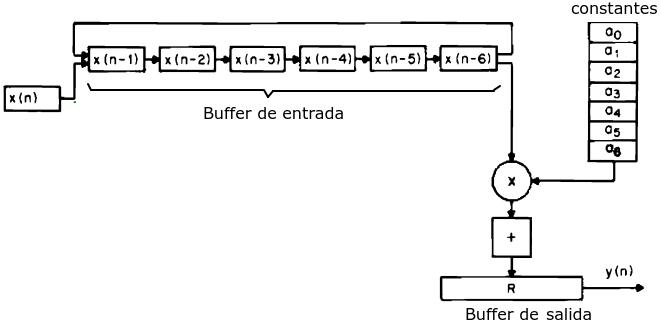
\includegraphics[scale=0.7]{procesamiento_micro_solo.jpg}	
	\caption{Representación del algoritmo de un filtro FIR}
	\label{fig:disenio_y_construccion:stm32:algoritmo}
	\end{figure}


Si bien el módulo ADC tiene como características de soportar casi 2 MSPS, intervienen otros factores que hacen que se reduzcan la tasa de muestreo. El factor preponderante es la cantidad de ciclos de reloj que lleva el procesamiento del algoritmo del filtro, compuestos por multiplicaciones, acumulaciones, actualización de registros; este tiempo se incrementa proporcional a la cantidad de términos que tenga el filtro a procesar. Cuanto más sea el orden del filtro, mayor cantidad de términos tendrá y mayor cantidad de operaciones computacionales tendrá que ejecutar.\newpage


\textbf{Implementación realizada utilizando matriz de puertas lógicas programables, FPGA}\\

El montaje completo consiste en la utilización de una placa de desarrollo FPGA y un circuito R2R, Fig. \ref{fig:disenio_y_construccion:fpga:board}.
\begin{figure}
	\centering
	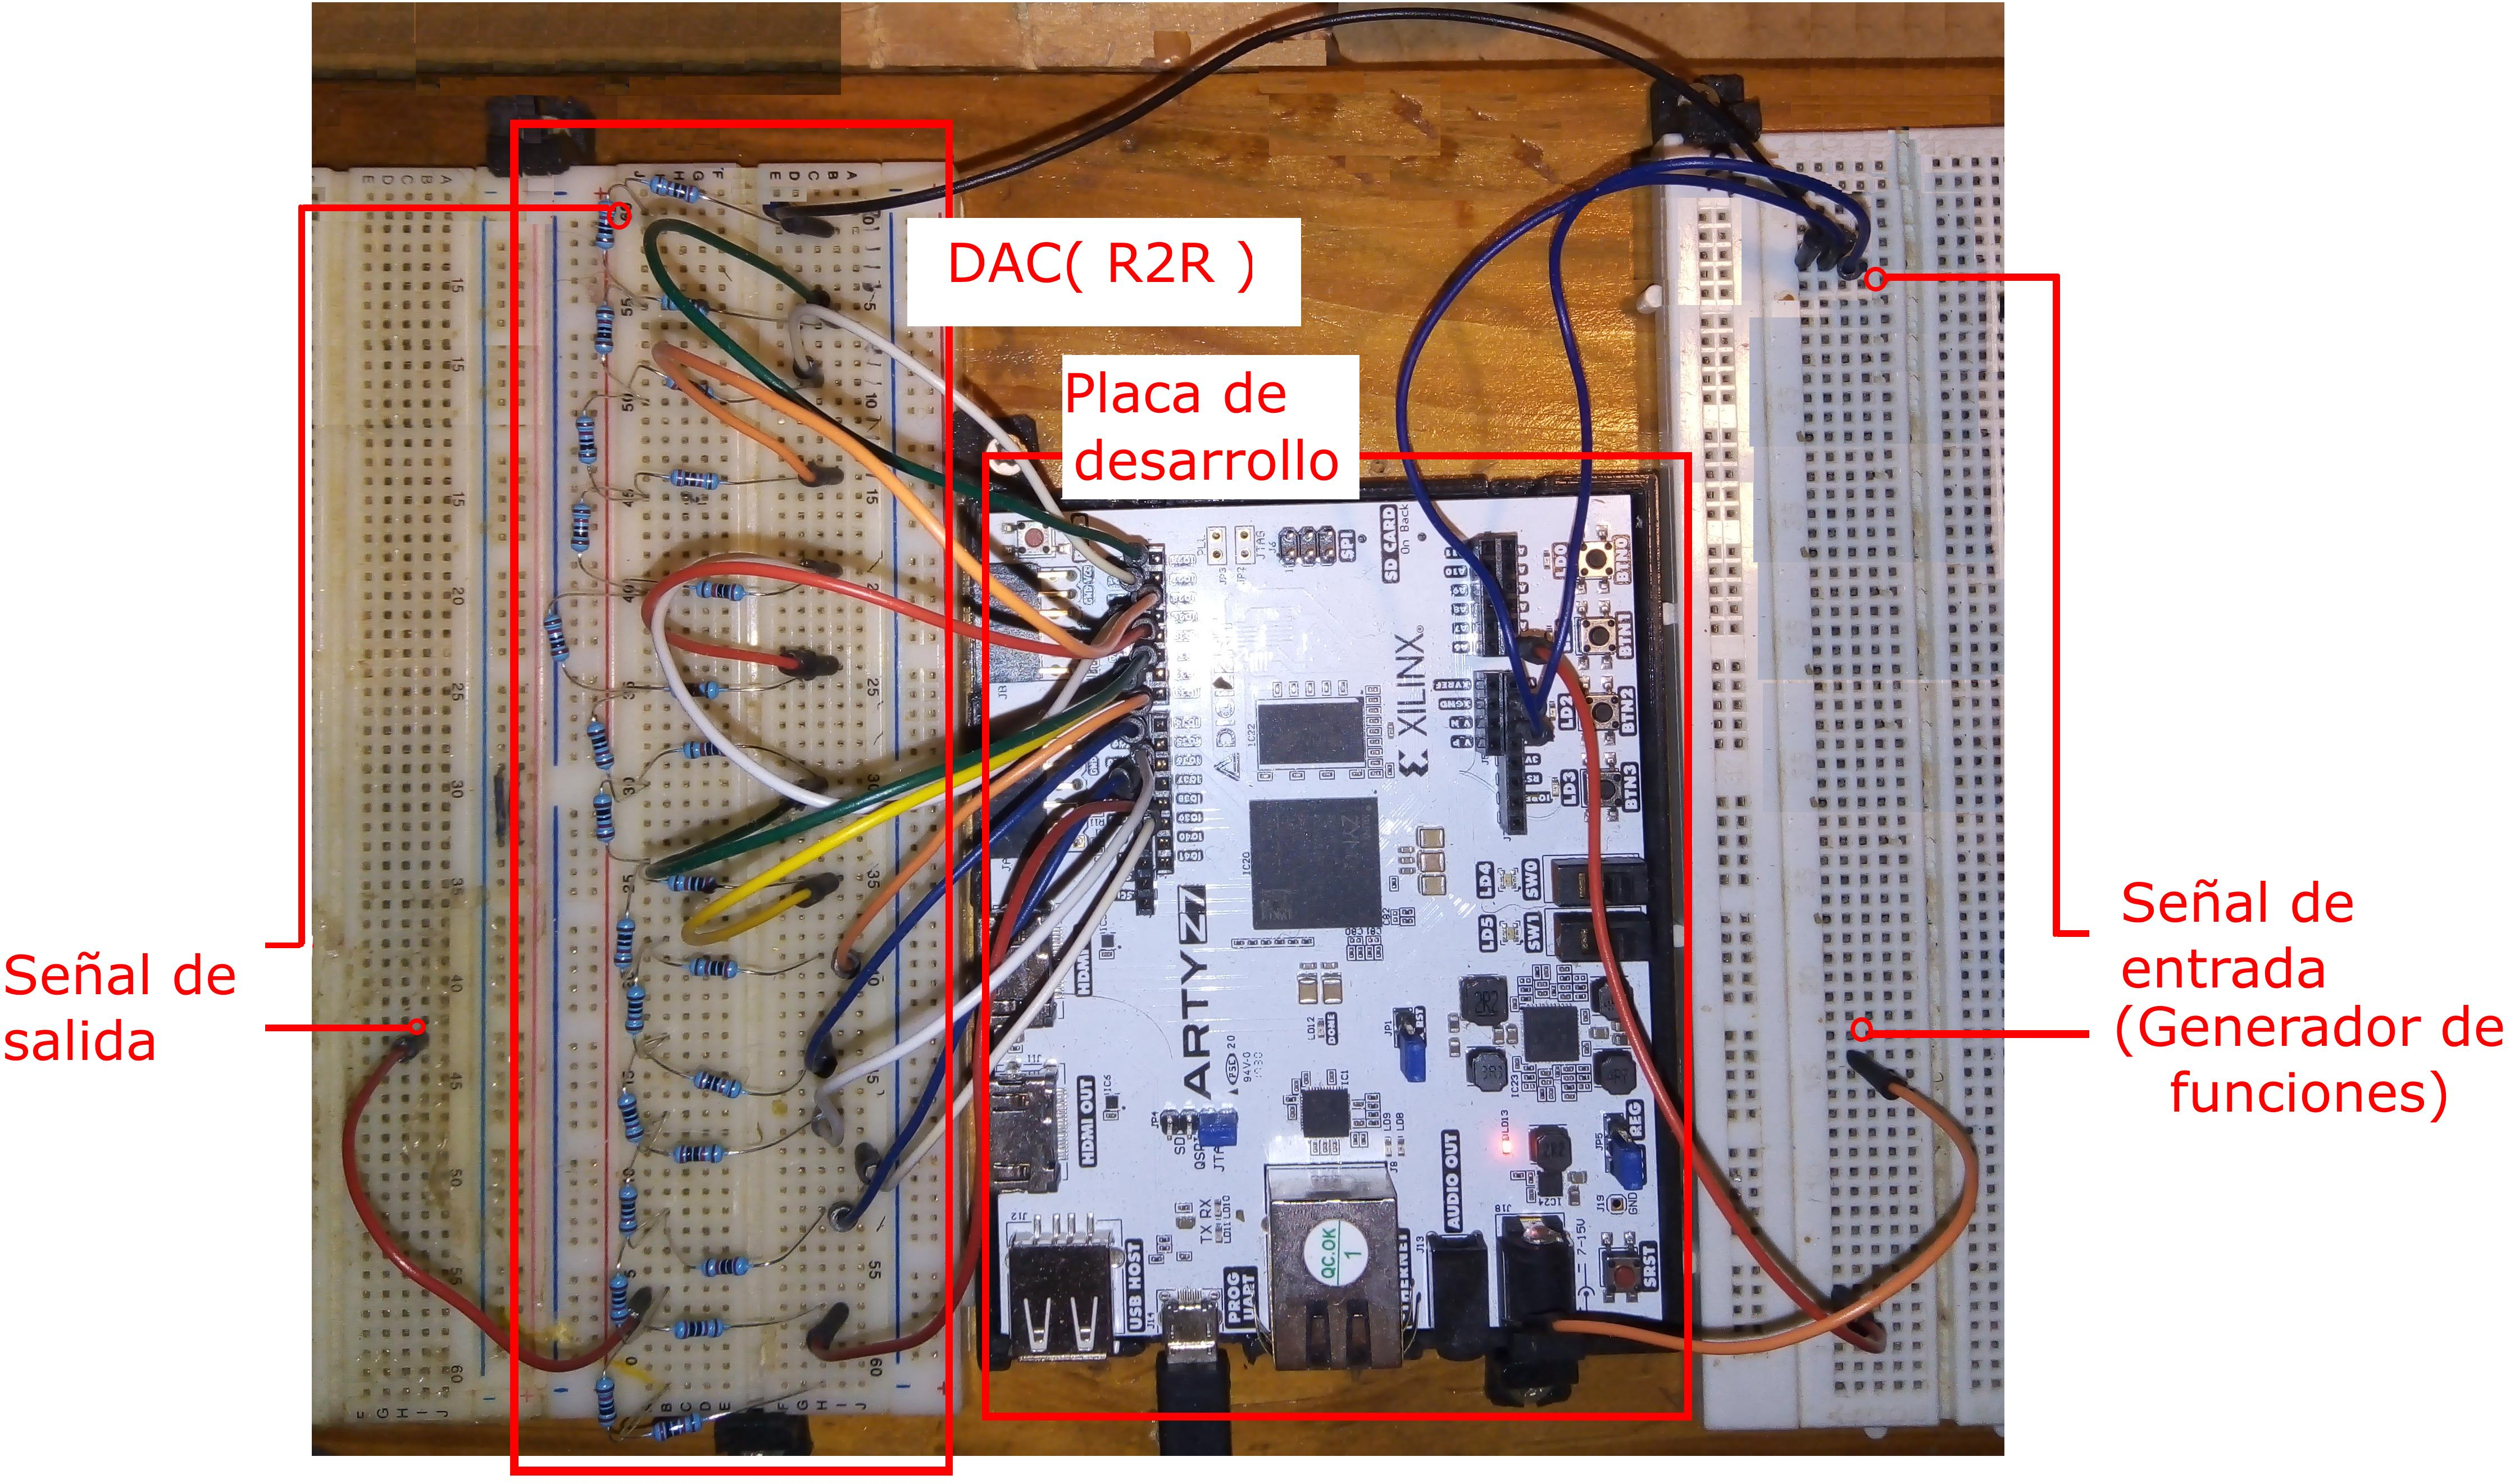
\includegraphics[scale=0.10]{foto_fpga_board.jpg}	
	\caption{Montaje del sistema embebido con FPGA}
	\label{fig:disenio_y_construccion:fpga:board}
	\end{figure}
La placa de desarrollo utilizada pertenece a la serie Arty Z7, fabricada por Digilent, contiene un chip programable de la linea Zynq-7000 de Xilinx denominado Arty Z7-20 XCZ020-1CLG400C. Este chip trae las siguientes capacidades:\newline

1- Un ADC integrado de 12bits y de 1MSPS, tiene entrada diferenciales. La placa deja accesible 6 puertos analógicos de forma diferencial y 4 mediante una adaptación que convierte la entrada a unipolar. EL voltaje máximo de entrada en modo diferencial es de 1Vpp, y para el modo unipolar es de 0 de 3.3V.\newline 
	
2 - El integrado trae otros módulos, como el generador de señal de reloj, microprocesadores, etc. Entre estos el integrado contiene una FPGA compuesto de 53200 LUTs y 106400 Flip-Flops.\\\\

En cuanto a la entrada analógica utilizada, se usó las entradas unipolares, Fig. \ref{fig:disenio_y_construccion:fpga:board:xadc}. Ésta tiene una frecuencia máxima de entrada de 100 MHz.\newline

\begin{figure}[h]
	\centering
	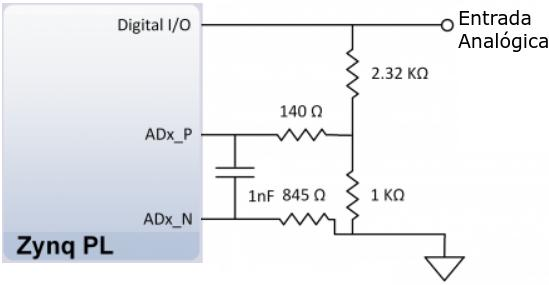
\includegraphics[scale=0.5]{fpga_xadc.jpg}	
	\caption{Circuito de entrada analógica unipolar incluido en la placa embebida utilizada}
	\label{fig:disenio_y_construccion:fpga:board:xadc}
	\end{figure}

Esta placa de desarrollo, no trae el modulo de conversión digital a analógico, para compensar, la empresa que manufactura la placa sugiere la utilización de un R2R, Fig. \ref{fig:disenio_y_construccion:fpga:board:r2r}.\\

\begin{figure}[h]
	\centering
	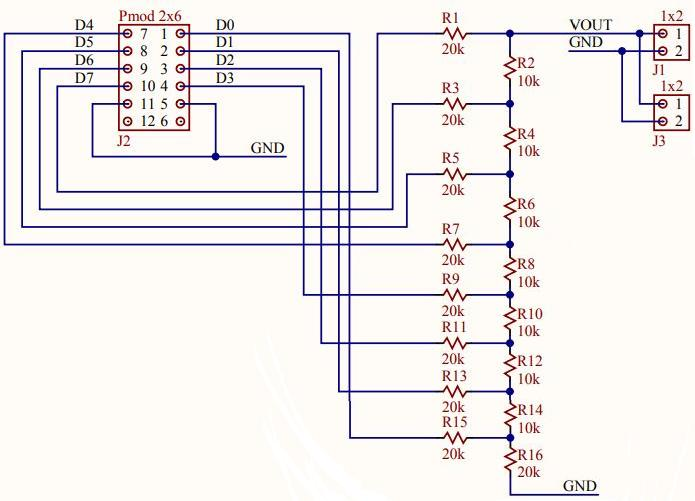
\includegraphics[scale=0.6]{fpga_dac_r2r.jpg}	
	\caption{Circuito R2R sugerido por la empresa que manufactura la placa embebida}
	\label{fig:disenio_y_construccion:fpga:board:r2r}
	\end{figure}
	
Al igual que la implementación realizada con microcontrolador, la arquitectura del filtro se puede resumir en la siguiente Fig. \ref{fig:disenio_y_construccion:fpga:board:arq}. En la Fig. \ref{fig:disenio_y_construccion:fpga:board:arq} muestra de forma abreviada la construcción de un filtro. 

\begin{figure}[h]
	\centering
	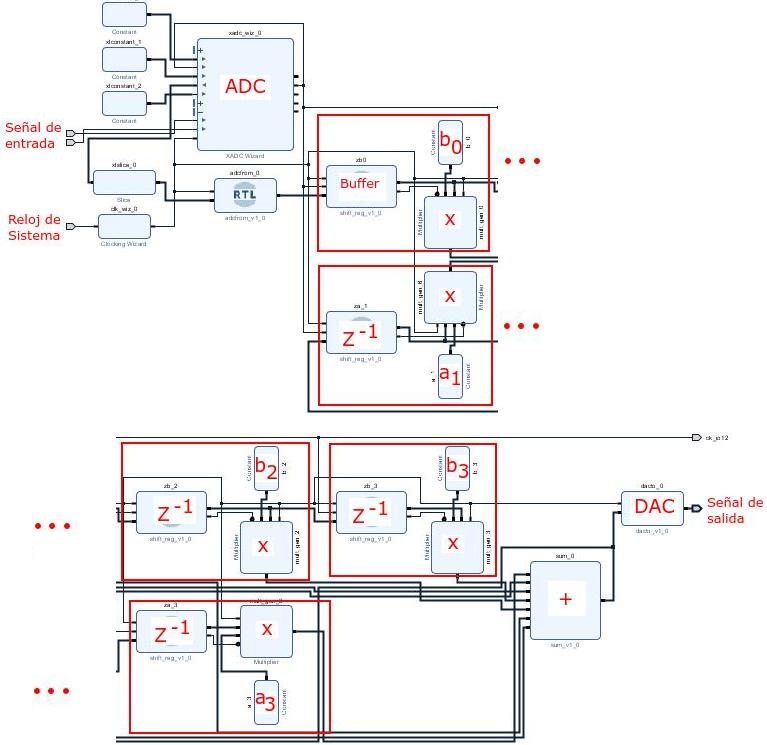
\includegraphics[scale=0.8]{fpga_arq_filtro_xilinx.jpg}	
	\caption{Representación de filtro realizado con FPGA mediante los bloques construidos para tal fin}
	\label{fig:disenio_y_construccion:fpga:board:arq}
	\end{figure}


\end{document}	